196. \begin{figure}[ht!]
\center{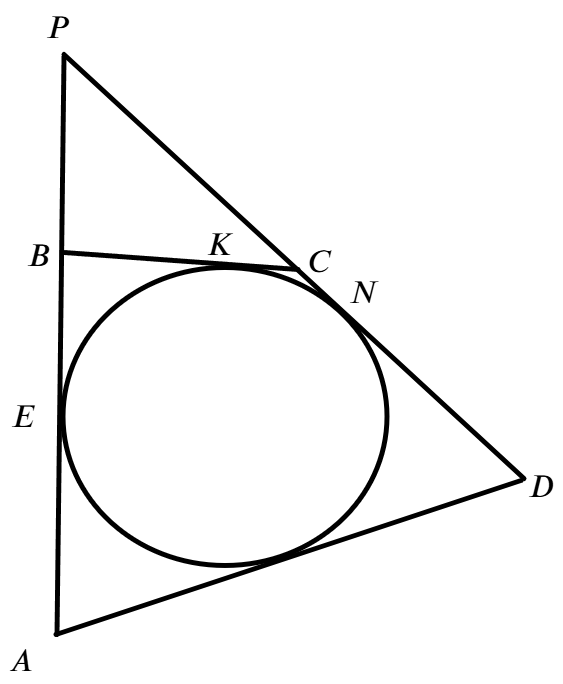
\includegraphics[scale=0.35]{g9-196.png}}
\end{figure}\\
Так как отрезки касательных, проведённых из одной точки, равны, имеем равенства $BE=BK,$ $CK=CN,\ PE=PN,$ откуда $P_{\Delta BCP}=PB+PC+BC=PB+PC+BK+CK=
PB+PC+BE+CN=PE+PN=2EP=8$ и $EP=8:2=4.$\\
